\documentclass[12pt,a4paper]{article}
\usepackage{graphicx}
\usepackage{hyperref}
\title{ProcessSchedulinginOperatingSystemsandEvolutionofWindows2023 — Research Booklet}
\date{}
\begin{document}
\maketitle
\tableofcontents
\newpage
\section{CITATIONS}
There is no section to summarize. The input is just a single digit "0". If you meant to provide a section of text, please feel free to paste it, and I'll be happy to help you summarize it in clear and simple terms!

Further reading: https://www.semanticscholar.org/search?q=CITATIONS
\begin{figure}[h]
\centering
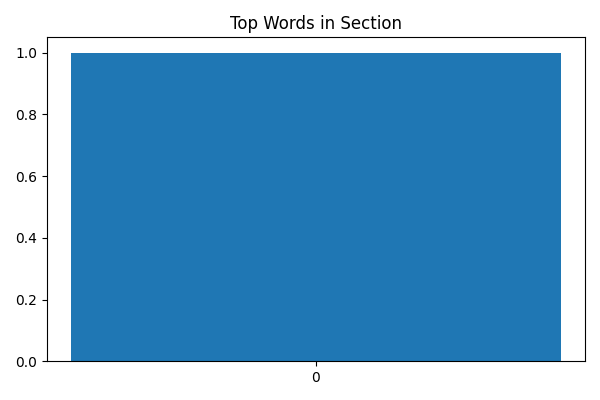
\includegraphics[width=0.8\textwidth]{D:\projects\mp 2 rag\autonomous rag\outputs\visual_bf653c5376a642c4b34e7f8fa555eb3e.png}
\end{figure}
\section{READS}
Here is a summary of the section in clear, simple terms:

Armaan Sidhu is a researcher from Manipal University Jaipur. He has written 4 publications (like articles or papers) and has been cited (referenced) 14 times by others.

Further reading: https://www.semanticscholar.org/search?q=READS
\begin{figure}[h]
\centering
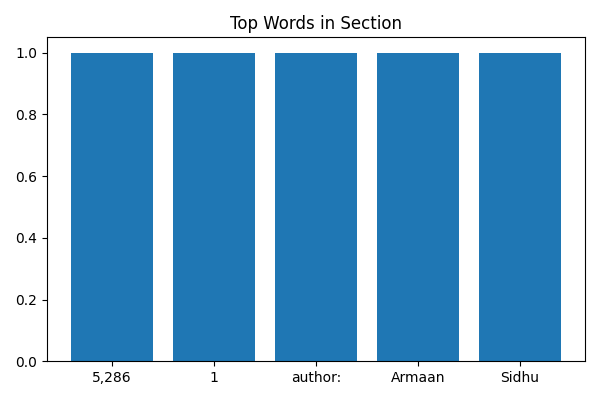
\includegraphics[width=0.8\textwidth]{D:\projects\mp 2 rag\autonomous rag\outputs\visual_04bee7ca787a4465b8ef58dbaa0e14a9.png}
\end{figure}
\section{SEE PROFILE}
Here's a summary of the section in clear and simple terms:

This is a technical paper about how operating systems manage the use of the computer's processor (CPU) by different programs or "processes". The paper focuses on how the Windows operating system does this, and how it has improved over time.

The paper explains that the process of deciding which program gets to use the CPU and for how long is called "process scheduling". This is important because it affects how well the computer performs and how quickly it can do tasks.

There are different ways that operating systems can schedule processes, and each method has its own strengths and weaknesses. The Windows operating system has changed its scheduling method over the years to make it faster and better at handling multiple programs at the same time.

The paper will provide a detailed understanding of process scheduling in operating systems, and how Windows has improved its scheduling method over time. This information will be useful for students, researchers, and professionals who work on designing and developing operating systems.

Further reading: https://arxiv.org/search/?query=SEE+PROFILE&searchtype=all
\begin{figure}[h]
\centering
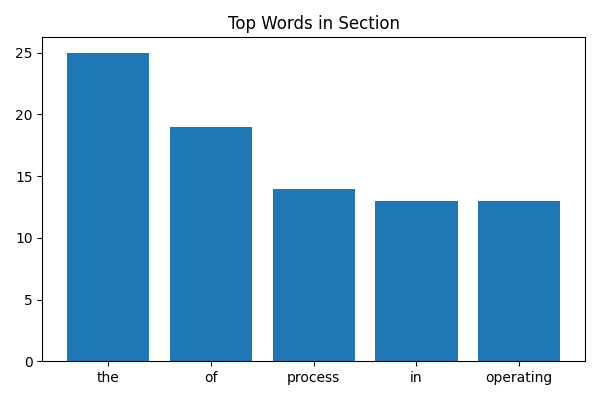
\includegraphics[width=0.8\textwidth]{D:\projects\mp 2 rag\autonomous rag\outputs\visual_ebb4e03c5c784e1daa9c14f23e696bed.png}
\end{figure}
\section{P}
Here's a summary of the section in clear and simple terms:

**Process Scheduling in Windows**

In the past, Windows used a simple algorithm to give each process a turn to use the CPU. However, as more processes were added, this algorithm wasn't efficient. So, Windows 95 introduced a new algorithm that prioritized processes based on their importance. This improved the system's performance and responsiveness.

Over time, Windows continued to improve its process scheduling algorithm to handle more complex tasks. For example, Windows Vista considered the number of threads associated with a process when making scheduling decisions.

**What is Process Scheduling?**

Process scheduling is the technique of assigning computer resources, like CPU time, to different processes that are competing for it. There are two main types of process scheduling algorithms: preemptive and non-preemptive.

**Preemptive Scheduling**

In preemptive scheduling, the CPU can be interrupted and assigned to another process at any time. This type of scheduling is complex and requires more data structures and algorithms.

**Non-Preemptive Scheduling**

In non-preemptive scheduling, a process uses the CPU until it completes its task or releases the CPU voluntarily. This type of scheduling is simple and doesn't require complex data structures.

**Process States**

A process goes through different states during its lifetime, including:

* New: The process is being created.
* Ready: The process is loaded into memory and waiting for the CPU to execute its instructions.
* Run: The process is being executed by the CPU.
* Blocked: The process is waiting for an I/O operation to complete.
* Terminated: The process has finished its task.

**Types of Process Schedulers**

There are three types of process schedulers:

* Long-term scheduler: responsible for selecting processes to be loaded into memory.
* Medium-term scheduler: responsible for swapping processes in and out of memory.
* Short-term scheduler: responsible for selecting the next process to be executed by the CPU.

Further reading: https://arxiv.org/search/?query=P&searchtype=all
\begin{figure}[h]
\centering
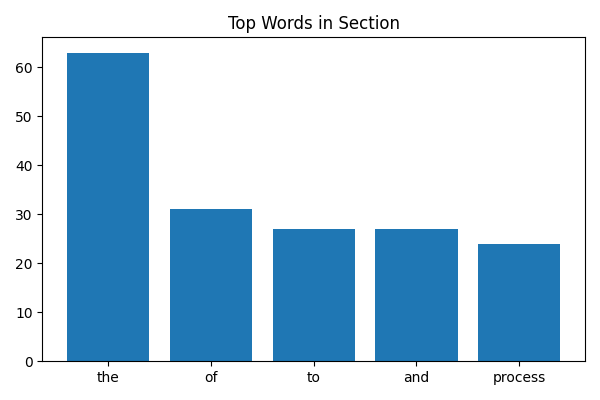
\includegraphics[width=0.8\textwidth]{D:\projects\mp 2 rag\autonomous rag\outputs\visual_4f3f705df4334aa1b269ae5f6552084b.png}
\end{figure}
\section{1. Long-Term Scheduler: The Long-Term Scheduler, also}
Here's a simple summary:

The Job Scheduler (also called the long-term scheduler) is in charge of choosing which programs to run on the computer and when. It decides which programs can start running and which ones have to wait. It looks at things like how busy the computer is, how much memory and input/output (like keyboard and screen) each program needs, and how important each program is. Its main goal is to pick a good mix of programs to run at the same time, so the computer can do its job efficiently and get as much work done as possible.

Further reading: https://www.semanticscholar.org/search?q=1.%20Long-Term%20Scheduler:%20The%20Long-Term%20Scheduler,%20also
\begin{figure}[h]
\centering
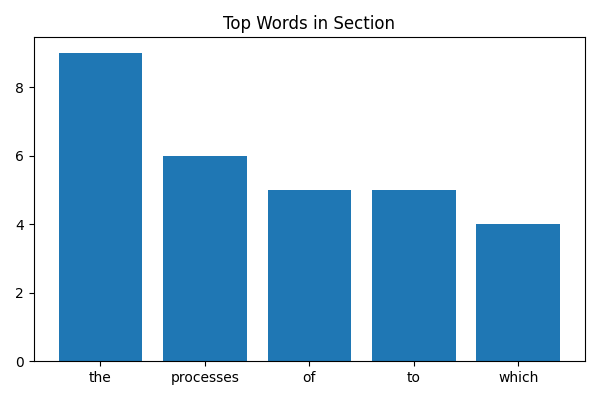
\includegraphics[width=0.8\textwidth]{D:\projects\mp 2 rag\autonomous rag\outputs\visual_d8c2bb6c46b540508cbf43b93791f3d2.png}
\end{figure}
\section{2. Medium-Term Scheduler: The Medium-Term Scheduler,}
Here's a simple summary:

The medium-term scheduler is a part of the operating system that helps manage memory. It does this by swapping processes (programs) in and out of memory. When a process is swapped out, its data is saved to the hard drive. When it's swapped back in, the data is restored from the hard drive. This helps free up memory for new processes that need to run. It also controls how many processes can run at the same time. Not all operating systems have this feature, but it's useful in systems with limited memory.

Further reading: https://www.semanticscholar.org/search?q=2.%20Medium-Term%20Scheduler:%20The%20Medium-Term%20Scheduler,
\begin{figure}[h]
\centering
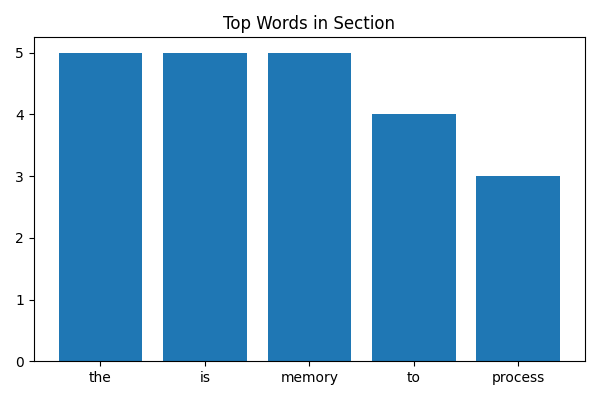
\includegraphics[width=0.8\textwidth]{D:\projects\mp 2 rag\autonomous rag\outputs\visual_7a41291d7f504721a90d2ad11a8bf917.png}
\end{figure}
\section{3. Short-Term Scheduler: The Short-Term Scheduler, also}
Here's a summary of the section in clear and simple terms:

**The CPU Scheduler**

The CPU scheduler is like a manager that decides which process (task) should use the computer's brain (CPU) next. It chooses from a list of processes that are ready to go and wants to make sure the CPU is always busy doing something. It uses different methods like "round-robin" or "shortest job first" to decide which process to pick.

**Three Types of Process Schedulers**

There are three types of schedulers that work together to manage the computer's resources:

1. Long-term scheduler: decides which new processes to add to the list
2. Medium-term scheduler: manages the memory by swapping processes in and out
3. Short-term scheduler: chooses which process to run on the CPU next

**Scheduling Algorithms**

Scheduling algorithms are like recipes that decide which process should run next and for how long. There are two main types:

1. Preemptive: allows the system to interrupt a running process and switch to a higher priority one
2. Non-preemptive: runs the current process to completion before switching to the next one

Choosing the right algorithm is important for good system performance. One common algorithm is priority scheduling, which assigns a priority level to each process based on factors like how long it's been waiting or how important it is to the system. The process with the highest priority level runs first.

Further reading: https://www.semanticscholar.org/search?q=3.%20Short-Term%20Scheduler:%20The%20Short-Term%20Scheduler,%20also
\begin{figure}[h]
\centering
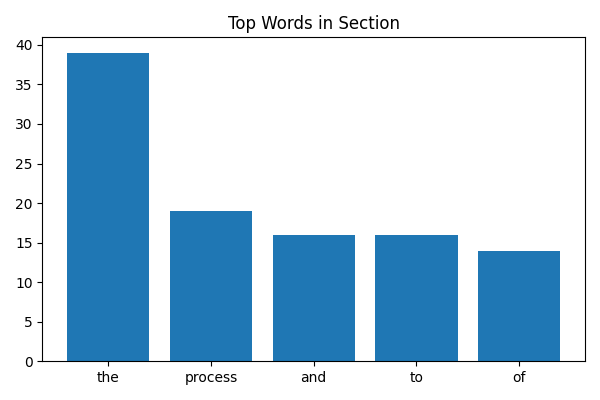
\includegraphics[width=0.8\textwidth]{D:\projects\mp 2 rag\autonomous rag\outputs\visual_4fa372b6906a48d59dd4862d80a41082.png}
\end{figure}
\section{2023. 
 
B. Longest Remaining Job First (LRJF)}
Here's a summary of the section in clear and simple terms:

**LRJF (Longest Remaining Job First)**

* A scheduling algorithm that chooses the process with the longest remaining execution time to run next.
* Good for batch processing environments where there's no interactive user, and for systems that require long execution times (e.g., scientific simulations).
* Not suitable for systems with a mix of long and short processes, as short processes might starve (wait a long time).

**SRJF (Shortest Remaining Job First)**

* A scheduling algorithm that chooses the process with the shortest remaining execution time to run next.
* Good for systems with a mix of long and short processes, as it minimizes waiting time.
* Not suitable for batch processing environments where long processes need to run.

**Round Robin (RR)**

* A scheduling algorithm that gives each process a fixed time slice (called a "time quantum") to run.
* When the time slice is up, the process is paused, and the next process in line gets a turn.
* Good for time-sharing systems where multiple users share a single system, as it ensures fair CPU time distribution.
* Simple to implement, but can have limitations like context switching overhead.

**FCFS (First Come – First Serve)**

* A scheduling algorithm that runs processes in the order they arrive.
* Simple to implement, but can lead to long waiting times for processes with longer execution times.
* Good for environments where processes have similar execution times and no prioritization is needed.
* Not suitable for systems with varying execution times and priorities.

In summary, each scheduling algorithm has its strengths and weaknesses, and the right choice depends on the system's requirements and workload.

Further reading: https://www.semanticscholar.org/search?q=2023.%20
%20
B.%20Longest%20Remaining%20Job%20First%20(LRJF)
\begin{figure}[h]
\centering
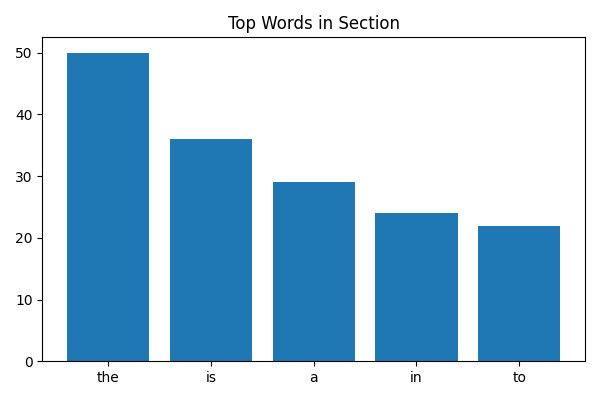
\includegraphics[width=0.8\textwidth]{D:\projects\mp 2 rag\autonomous rag\outputs\visual_d902258721e44362b37a26715bedf129.png}
\end{figure}
\section{5. 
FCFS}
Here's a simplified summary of the section:

**Scheduling Algorithms**

There are different ways that computer operating systems can schedule tasks to run efficiently. Here are a few examples:

* **Shortest Job First (SJF)**: This algorithm prioritizes tasks based on how long they take to complete. It's useful in environments where there's no interactive user, but it can have limitations, such as longer tasks monopolizing the CPU.
* **Longest Job First (LJF)**: This algorithm prioritizes tasks based on how long they take to complete, but in reverse order. It's useful in environments with long-running jobs, but may not be suitable for systems with a mix of long and short tasks.
* **Highest Response Ratio Next (HRRN)**: This algorithm prioritizes tasks based on their response ratio, which takes into account how long a task has been waiting and how long it takes to complete. It's useful in environments with varying execution times and waiting times.

**Evolution of Windows Operating System**

The Windows operating system has undergone significant changes and improvements over the years, from its first version in 1985 to the latest version, Windows 11, in 2021. Each new version has introduced new features, addressed issues from previous versions, and improved performance.

Let me know if you'd like me to clarify anything!

Further reading: https://arxiv.org/search/?query=5.+
FCFS&searchtype=all
\begin{figure}[h]
\centering
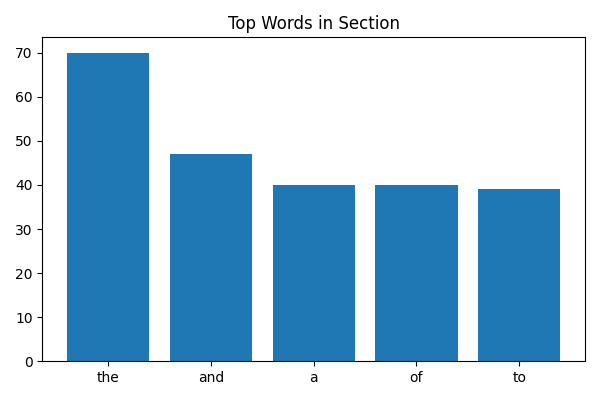
\includegraphics[width=0.8\textwidth]{D:\projects\mp 2 rag\autonomous rag\outputs\visual_0e8cae31a30b4f9186e1b2ed71d767c7.png}
\end{figure}
\section{ALGORITHMS}
This section compares and contrasts the different process scheduling algorithms used today, in a clear and concise way.

Further reading: https://www.semanticscholar.org/search?q=ALGORITHMS
\begin{figure}[h]
\centering
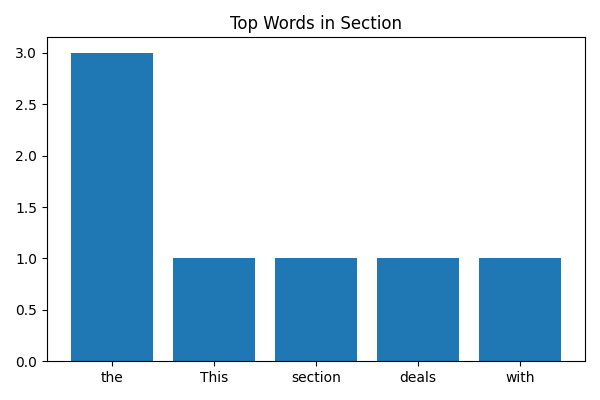
\includegraphics[width=0.8\textwidth]{D:\projects\mp 2 rag\autonomous rag\outputs\visual_abc4659fa7f442e7abfb4f29807efd54.png}
\end{figure}
\section{TABLE I}
Please provide the section you'd like me to summarize, and I'll do my best to break it down into clear and simple terms.

Further reading: https://scholar.google.com/scholar?q=TABLE+I
\begin{figure}[h]
\centering
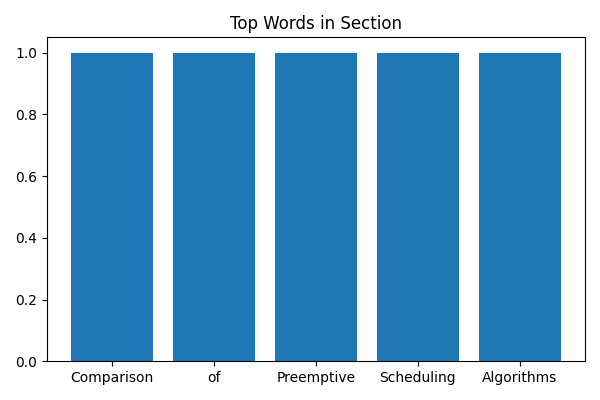
\includegraphics[width=0.8\textwidth]{D:\projects\mp 2 rag\autonomous rag\outputs\visual_80d75c0417024b5ca0f34dfe8f6bffcd.png}
\end{figure}
\section{TABLE II}
Here's a summary of the section in clear and simple terms:

Process scheduling is an important part of an operating system that helps manage how the computer's resources are shared among different tasks. The Windows operating system has improved its process scheduling over the years to make the computer run more efficiently and respond quickly to user input. From simple scheduling methods to more advanced ones, Windows has added new features to prioritize important tasks and allocate resources fairly. As computers continue to evolve, process scheduling will remain crucial to ensure that resources are used efficiently and tasks are completed smoothly.

Further reading: https://scholar.google.com/scholar?q=TABLE+II
\begin{figure}[h]
\centering
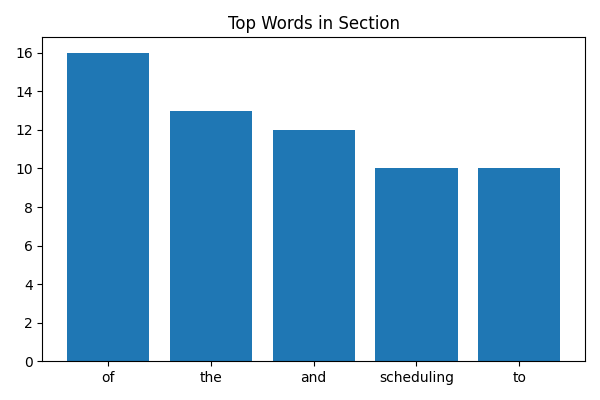
\includegraphics[width=0.8\textwidth]{D:\projects\mp 2 rag\autonomous rag\outputs\visual_d51383db09af4bafb9f3dd3806b7eb2c.png}
\end{figure}
\section{APPENDIX}
Here's a summary of the section in clear and simple terms:

**Computer Basics**

* A **process** is a program that is currently running on a computer.
* The **CPU** (Central Processing Unit) is the part of the computer that does the actual work of running programs.
* **Process scheduling** is how the computer decides which program to run next on the CPU.

**Scheduling Algorithms**

* A **scheduling algorithm** is a set of rules that determines the order in which programs are run on the CPU.
* There are two types of scheduling algorithms:
	+ **Preemptive**: allows a more important program to interrupt a less important one that's currently running.
	+ **Non-preemptive**: lets a program finish running before starting another one.

**Types of Scheduling Algorithms**

* **First Come First Serve (FCFS)**: runs programs in the order they arrive.
* **Shortest Job First (SJF)**: runs the program that will take the least amount of time to complete.
* **Longest Job First (LJF)**: runs the program that will take the most amount of time to complete.
* **Priority Scheduling**: runs the most important program first.
* **Round Robin (RR)**: gives each program a set amount of time to run before switching to the next one.

**Performance Measures**

* **Response time**: how long it takes for the computer to start running a program after it's submitted.
* **Throughput**: how many programs the computer can complete in a certain amount of time.
* **Fairness**: how well the computer shares its resources among all programs.

Further reading: https://www.semanticscholar.org/search?q=APPENDIX
\begin{figure}[h]
\centering
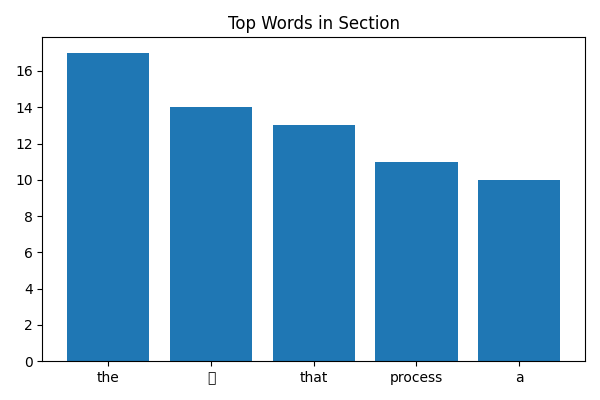
\includegraphics[width=0.8\textwidth]{D:\projects\mp 2 rag\autonomous rag\outputs\visual_a9a020ac376f46508b7ecffc7f2dd2a2.png}
\end{figure}
\section{REFERENCES AND FOOTNOTES}
This section lists the sources used in a document or research paper. These sources include:

* Three textbooks about operating systems:
	+ "Operating System Concepts" by Silberschatz, Galvin, and Gagne
	+ "Modern Operating Systems" by Tanenbaum and Bos
	+ "Operating Systems: Internals and Design Principles" by Stallings
* Two online articles from Microsoft's website:
	+ "Windows 11: Features and System Requirements"
	+ "A history of Windows"
* A technical standard from the Institute of Electrical and Electronics Engineers (IEEE) about the POSIX operating system interface.

There are no footnotes in this section.

Further reading: https://arxiv.org/search/?query=REFERENCES+AND+FOOTNOTES&searchtype=all
\begin{figure}[h]
\centering
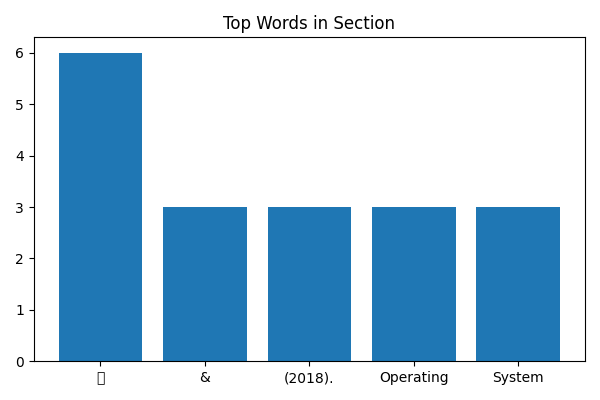
\includegraphics[width=0.8\textwidth]{D:\projects\mp 2 rag\autonomous rag\outputs\visual_cebbc0a7ba6f48ee91ca95103cb58789.png}
\end{figure}
\section{1. Windows 10 introduced several new features,}
This section is talking about two features of a computer system:

1. **Virtual Desktops**: This allows you to have multiple "desktops" on your computer, so you can organize your work and apps into separate spaces.
2. **Cortana Voice Assistant**: This is a feature that lets you talk to your computer and it will do things for you, like answer questions or set reminders.

Further reading: https://www.semanticscholar.org/search?q=1.%20Windows%2010%20introduced%20several%20new%20features,
\begin{figure}[h]
\centering
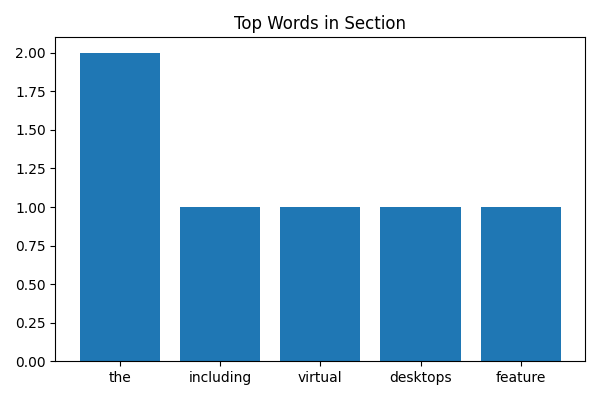
\includegraphics[width=0.8\textwidth]{D:\projects\mp 2 rag\autonomous rag\outputs\visual_edcbe2d8ed3f409cb6456a3d82950a0d.png}
\end{figure}
\section{2. In "Shortest Remaining Job First" scheduling, the}
Here's a simple summary:

The scheduler chooses the process that needs the least amount of time to finish its task to run next.

Further reading: https://arxiv.org/search/?query=2.+In+"Shortest+Remaining+Job+First"+scheduling,+the&searchtype=all
\begin{figure}[h]
\centering
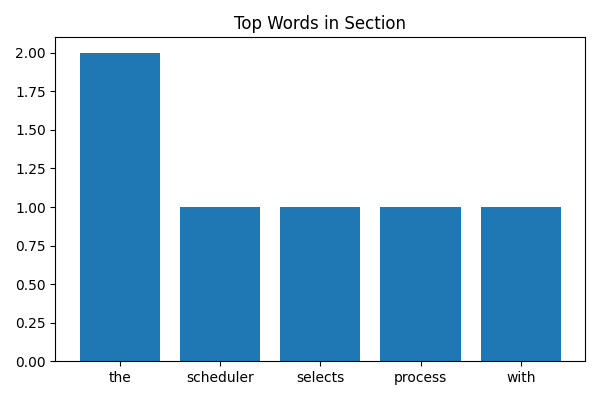
\includegraphics[width=0.8\textwidth]{D:\projects\mp 2 rag\autonomous rag\outputs\visual_05b5ccce190b46d0bcf53baacc402d1f.png}
\end{figure}
\section{3. In "Round Robin" scheduling, each process is}
Here's a simple summary:

Each process gets a turn to run for a short, fixed amount of time (called a "time slice" or "quantum"). When that time is up, the process is stopped and the next process in line takes its turn.

Further reading: https://arxiv.org/search/?query=3.+In+"Round+Robin"+scheduling,+each+process+is&searchtype=all
\begin{figure}[h]
\centering
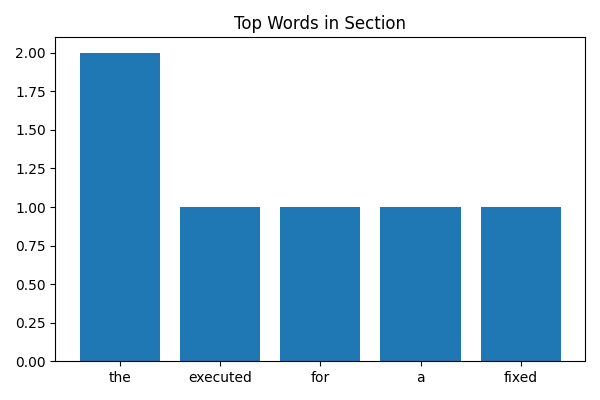
\includegraphics[width=0.8\textwidth]{D:\projects\mp 2 rag\autonomous rag\outputs\visual_48992f4d930f4aa3bee73b8b4faaaf14.png}
\end{figure}
\section{4. The term "time slice" refers to the amount of time}
Here is a summary of the section in clear, simple terms:

In Round Robin scheduling, each process gets a fixed amount of time (called a "time slice" or "time quantum") to run before the next process gets a turn.

Further reading: https://www.semanticscholar.org/search?q=4.%20The%20term%20"time%20slice"%20refers%20to%20the%20amount%20of%20time
\begin{figure}[h]
\centering
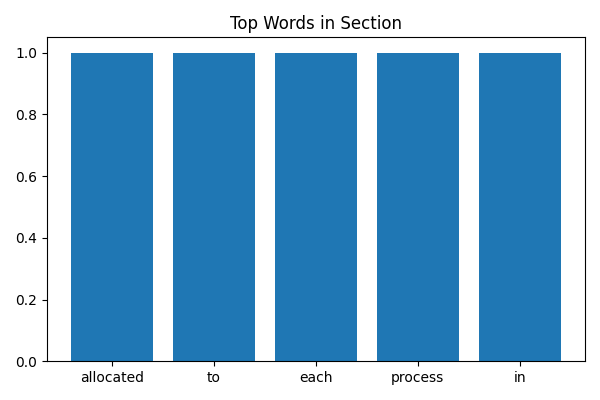
\includegraphics[width=0.8\textwidth]{D:\projects\mp 2 rag\autonomous rag\outputs\visual_37dd80364b0e47cc9414a801e772152a.png}
\end{figure}
\section{5. Windows Vista introduced several new features,}
This section is talking about two new things in a computer system:

1. A new way of looking at things on the screen, called "Aero glass interface", which makes things look nicer and more modern.
2. Some extra features to help keep your computer and information safe, called "enhanced security features".

Further reading: https://www.semanticscholar.org/search?q=5.%20Windows%20Vista%20introduced%20several%20new%20features,
\begin{figure}[h]
\centering
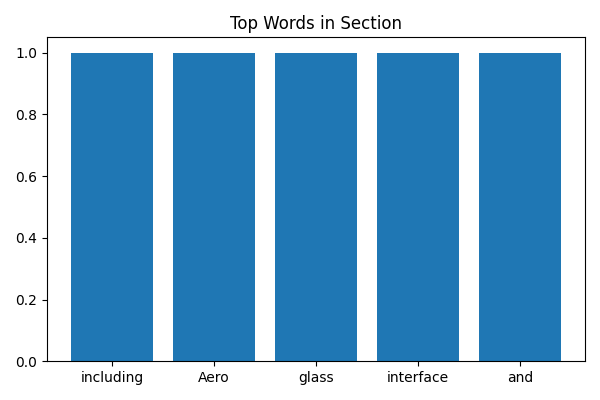
\includegraphics[width=0.8\textwidth]{D:\projects\mp 2 rag\autonomous rag\outputs\visual_9fd3a2c7c1e1443a8c9d5803992f6442.png}
\end{figure}
\section{6. The priority of a process can be adjusted dynamically}
Here is a summary of the section in clear, simple terms:

**Preemptive Priority Scheduling at Runtime**

When a computer program is running (during "runtime"), the operating system uses a scheduling method called Preemptive Priority Scheduling to decide which tasks to run and when.

Here's how it works:

* The operating system assigns a priority level to each task (or process) based on its importance.
* The task with the highest priority gets to run first.
* If a new task with a higher priority becomes available, the operating system can "preempt" (or interrupt) the current task and switch to the new one.
* This ensures that the most important tasks get done quickly and efficiently.

In short, Preemptive Priority Scheduling helps the operating system manage tasks efficiently and prioritize the most important ones during runtime.

Further reading: https://arxiv.org/search/?query=6.+The+priority+of+a+process+can+be+adjusted+dynamically&searchtype=all
\begin{figure}[h]
\centering
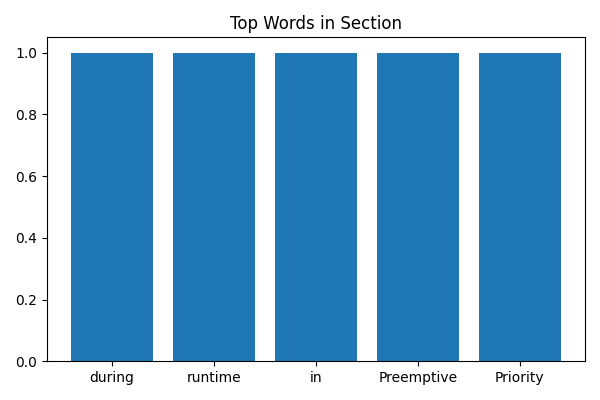
\includegraphics[width=0.8\textwidth]{D:\projects\mp 2 rag\autonomous rag\outputs\visual_8b07e7537fab4bb9a4b2153ed4923457.png}
\end{figure}
\section{7. The term "burst time" refers to the amount of time}
Here is a simple summary:

**CPU Scheduling algorithms** need to know how much **time** a process needs to **finish its task**.

Further reading: https://scholar.google.com/scholar?q=7.+The+term+"burst+time"+refers+to+the+amount+of+time
\begin{figure}[h]
\centering
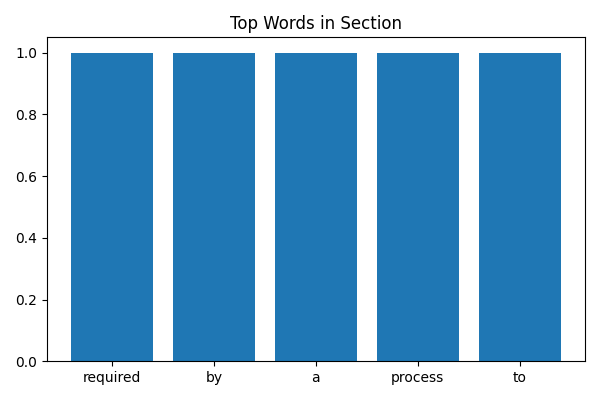
\includegraphics[width=0.8\textwidth]{D:\projects\mp 2 rag\autonomous rag\outputs\visual_3bc75fd295024817a974ff53bd16dbe9.png}
\end{figure}
\section{ACKNOWLEDGMENT}
Here's a simple summary of the section:

The author, Armaan Sidhu, is thanking everyone who helped him complete his technical article. He thanks his colleagues and mentors for their guidance and feedback, as well as the academic and research communities for their contributions to the field of cryptography. He also thanks the digital world for inspiring him to research and develop better operating systems.

The author then introduces himself, saying he's a computer science student at Manipal University Jaipur, with a focus on cyber security. He lists his work experience, including internships in web development and content writing. He's also a founding member of a club at his university that focuses on green computing, cyber security, and research.

Further reading: https://www.semanticscholar.org/search?q=ACKNOWLEDGMENT
\begin{figure}[h]
\centering
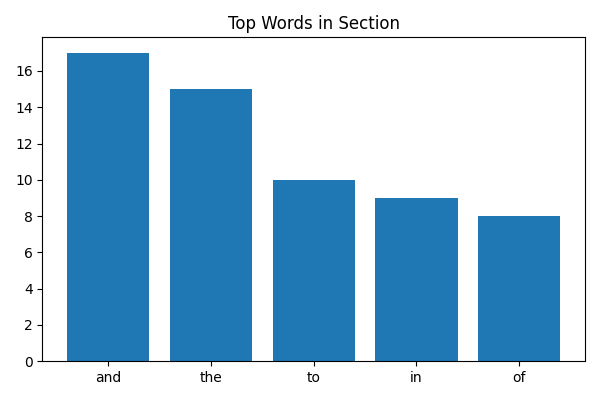
\includegraphics[width=0.8\textwidth]{D:\projects\mp 2 rag\autonomous rag\outputs\visual_906837cc7ea94cfe86b2d21851408c47.png}
\end{figure}
\end{document}